% !TeX root = ../main.tex
% !TeX encoding = UTF-8
% !TeX spellcheck = none

\section{Introduction}\label{sec:introduction}

Anticipating travel demand across urban regions supports fleet dispatch and the allocation of transport resources~\cite{ref44}. Regional inflow and outflow describe trips arriving in and departing from each region within a given interval~\cite{ref36}; their variation determines where demand concentrates, how large it becomes, and how long it persists. Dispatch decisions require forecasts of successive increases, decreases, and spatial shifts in demand to guide vehicle deployment and regional service provision~\cite{ref27,ref43}. Short-term multi-step traffic flow forecasting therefore jointly estimates regional inflow and outflow at successive future time steps from recent observations, supporting dispatch decisions over the next 5--60 minutes. \citationupdated{Traffic event information has been used to supplement historical traffic observations and improve short-term flow forecasting~\cite{ref42}}. Improving multi-step regional forecasting requires models to capture routine spatiotemporal patterns while responding to local changes in demand.

Traffic flow forecasting has progressed through advances in spatial dependency learning, temporal pattern representation, and multiscale dynamics modeling. For regional flow forecasting, ST-ResNet uses residual convolutions to jointly model temporal closeness, periodicity, and trends. In its single-step TaxiBJ experiment at a 30-minute resolution, the best configuration reduced RMSE from DeepST's 18.18 to 16.69, a relative decrease of approximately 8.2\%~\cite{ref14}. Spatiotemporal graph networks combine inter-node relations with temporal encoding, learning spatial dependencies through diffusion convolution, graph convolution, and adaptive adjacency matrices~\cite{ref01,ref02,ref03}. STWave and TEDDCF use frequency decomposition and two-branch encoding to represent low-frequency trends and high-frequency dynamics separately~\cite{ref11,ref18}. \citationupdated{ST-GDN further combines local geographic dependencies, global regional associations, and multiscale temporal attention to organize historical information~\cite{ref41}}. These studies broaden the historical information available to forecasting models, drawing on node trajectories, cross-region relations, and temporal patterns at different scales. When local flow deviates from routine patterns, however, the relevance of this historical evidence needs to be reassessed in light of the current state. Determining its relevance at different forecast horizons and translating it into effective prediction corrections remain important questions for short-term multi-step forecasting.

These issues concern both the sources of evidence and the conditions under which historical messages are useful. A node's own history directly records the continuation and turning points of its local state, whereas observations from other regions provide cross-region references through directed time-lagged associations~\cite{ref47}. These sources differ in their spatial origins, temporal alignment, and correction roles. Even for the same neighbor, historical messages correspond to different lag positions and scales of variation; \citationupdated{their relevance must be assessed using the source and target traffic backgrounds and the forecast horizon}. \editorialupdated{Figure~\ref{fig:intro-case} illustrates these differences using outflow from grid cell 601 in Chengdu in November 2016:} for two recent traffic states, the historical correlations between the target and a lag-aligned neighboring region were 0.859 and 0.907, respectively, whereas the mean absolute differences between their observed trajectories over the subsequent 30--60 minutes were 0.5 and 6.0 counts per 15 min. Both states exhibited strong historical associations but differed in how far their subsequent trajectories diverged. This observation focuses attention on the conditions under which historical information remains useful. Self-evolution and cross-region time-lagged evidence need distinct roles in correcting the base prediction, while historical messages need to be selected for each future forecast step according to the current background.

Existing approaches address heterogeneous dynamics and cross-region information through signal disentanglement, expert routing, and delay awareness. D2STGNN separates diffusion and inherent signals through gating and residual decomposition, then models them with different modules~\cite{ref25}. TESTAM uses temporal, static-graph, and dynamic-graph experts, adapting to different traffic conditions through routing~\cite{ref26}. PDFormer combines dynamic spatial attention with delay-aware feature transformations to address temporal misalignment in cross-region information~\cite{ref10}. These studies provide a basis for distinguishing sources of dynamics and establishing spatiotemporal associations, making the organization of prediction evidence more explicit. For multi-step regional forecasting under local deviations, linking such differentiated modeling to correction benefits requires understanding when self-evolution and directed time-lagged information improve the base prediction, and how the benefits of cross-region historical messages vary with source--target background discrepancy and forecast horizon.

\begin{figure}[!t]
	\centering
	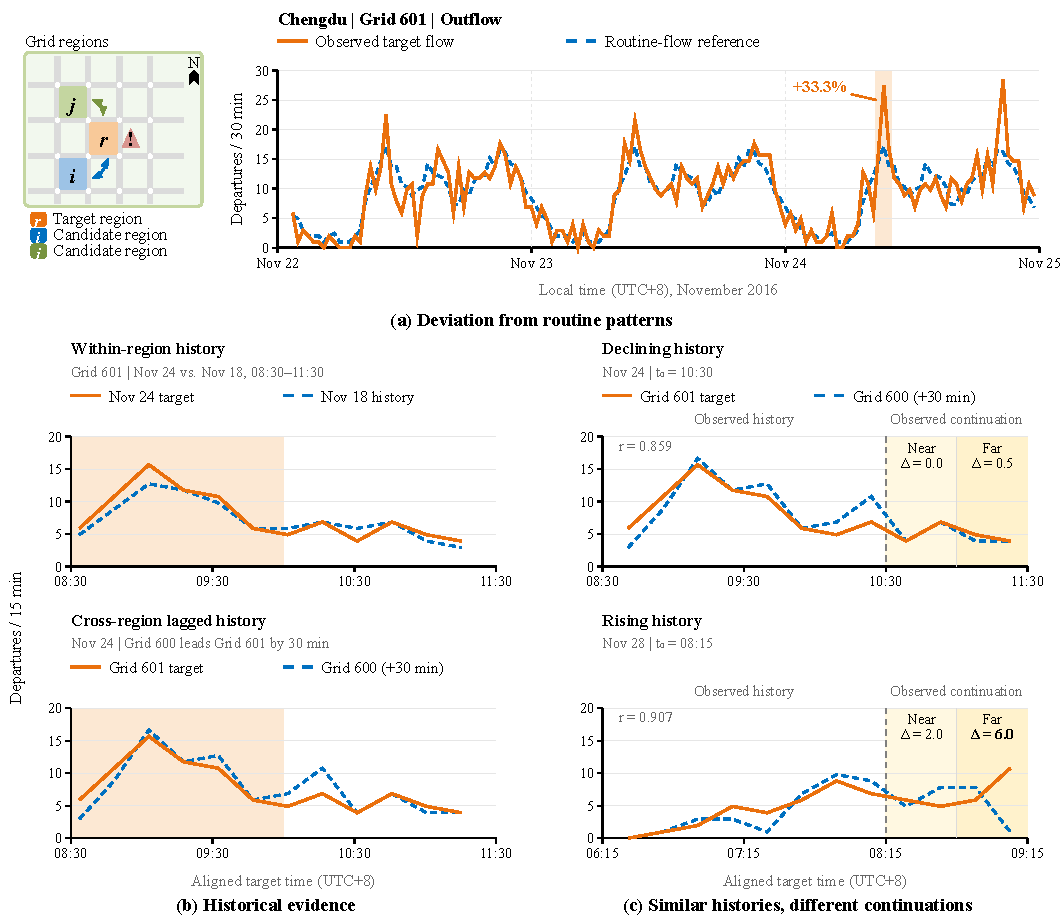
\includegraphics[width=\linewidth]{figures/introduction-case.pdf}
	\caption{\editorialupdated{Observed deviations from routine flow patterns and historical references. (a) Routine-flow reference and observed flow. (b) Within-region and cross-region historical evidence. (c) Divergent subsequent trajectories following similar histories.}}
	\label{fig:intro-case}
\end{figure}

We introduce the Role-aware and Background-conditioned Spatiotemporal Residual Network (RBSRN) to organize correction evidence and select historical messages when local flow deviates from routine patterns. RBSRN refines a base prediction through adaptive fusion of heterogeneous experts and background-conditioned selection of historical messages. Shared dual-frequency spatiotemporal encoding first extracts low- and high-frequency representations and generates the base prediction. The State-Evidence Expert Residual Refinement Module (SERR) assigns distinct roles to self-evolution and directed time-lagged experts and allocates their correction contributions according to the current state. Background-conditioned Cross-region Message Selection (BCMS) uses the low-frequency source and target traffic backgrounds to jointly select high-frequency historical messages for each forecast step. Both modules read the shared representations in parallel, and their corrections are added at the prediction stage to jointly forecast regional inflow and outflow over multiple future steps.

The main contributions are as follows:

\begin{enumerate}
	\def\labelenumi{\arabic{enumi}.}
	\item
	To account for heterogeneous prediction evidence and allocate its contributions under deviations from routine patterns, we introduce SERR. Its state-conditioned gate combines residual corrections from self-evolution and directed time-lagged experts to refine the base prediction according to the current state. \revised{Ablation experiments on Chengdu showed that removing either expert increased both MAE and RMSE for inflow and outflow.}
	\item
	To account for changes in the relevance of cross-region historical evidence across traffic backgrounds and forecast horizons, we introduce BCMS. It jointly selects neighbor--lag--scale messages for each forecast step, providing background-conditioned and horizon-specific residual corrections to the base prediction. Fixed-model residual-removal diagnostics in both cities showed larger average MAE benefits from these corrections when the history-derived proxy for background discrepancy between the target and candidate source regions was smaller.
	\item
	We systematically evaluated RBSRN's forecasting performance and residual refinement on the Chengdu and Shanghai datasets. In the overall comparison with 13 representative baseline methods, RBSRN achieved the lowest AVG12 MAE on all four city--channel forecasting tasks, reducing MAE by \shanghaiupdated{0.43\%}--2.00\% relative to each task's strongest baseline method. \shanghaiupdated{It also achieved the lowest AVG12 RMSE on all four tasks}.
\end{enumerate}
